%% REVISED MAIN.TEX - Major Revision for King Faysal Journal

\documentclass[pdflatex,sn-mathphys-num]{sn-jnl}

\usepackage{graphicx}%
\usepackage{multirow}%
\usepackage{amsmath,amssymb,amsfonts}%
\usepackage{amsthm}%
\usepackage{mathrsfs}%
\usepackage[title]{appendix}%
\usepackage{xcolor}%
\usepackage{textcomp}%
\usepackage{manyfoot}%
\usepackage{booktabs}%
\usepackage{algorithm}%
\usepackage{algorithmicx}%
\usepackage{algpseudocode}%
\usepackage{listings}%
\usepackage{subcaption}%
\usepackage{siunitx}%

\theoremstyle{thmstyleone}%
\newtheorem{theorem}{Theorem}%
\newtheorem{proposition}[theorem]{Proposition}% 

\theoremstyle{thmstyletwo}%
\newtheorem{example}{Example}%
\newtheorem{remark}{Remark}%

\theoremstyle{thmstylethree}%
\newtheorem{definition}{Definition}%

\raggedbottom

\newcommand{\methodname}{SC-PINN}
\newcommand{\baseline}{Standard PINN}
\newcommand{\softpinn}{Penalty-Based IP-PINN}
\providecommand{\vs}{vs.\ }

\begin{document}
	
	\title[Structurally Corrected Invariant-Preserving Neural Networks]{Structurally Corrected Invariant-Preserving Neural Networks for Conservative Dynamical Systems: A Statistically Validated Approach}
	
	\author*[1]{\fnm{Fatima} \sur{Ouaar}}\email{f.ouaar@univ-biskra.dz}
	\affil*[1]{\orgdiv{Mathematics Department}, \orgname{University of Biskra}, \orgaddress{\city{Biskra}, \postcode{07000}, \country{Algeria}}}
	
	\abstract{In this paper a structural correction in neural network architecture for the long-time integration of conservative dynamical systems is used to overcome uncontrolled invariant drift existing in standard physics-informed formulations. The Structurally Corrected IP-PINN is used to solve the Lotka--Volterra predator-prey system where the multiplicative architectural correction to the invariant manifold demonstrates from a statistical significance perspective improvements beyond both baseline and soft-constraint methods (Welch's $t$-test, $p < 10^{-11}$, Cohen's $d = 5.03$). Also our structurally corrected neural network (\methodname) reaches a \textbf{72.2\% reduction} in invariant drift (mean $9.54\times10^{-2}$ \vs{} $3.43\times10^{-1}$) contrasted to the baseline, and a \textbf{66.9\% improvement} over soft penalty techniques.}
	
	\keywords{Physics-informed neural networks, Invariant preservation, Structural correction, Conservative systems, Statistical validation}
	\pacs[MSC Classification]{37M05, 65P10, 65M70, 68T07}
	\maketitle
	
	\section{Introduction}\label{sec1}
	
	In numerical approximation there is a significant challenge regarding long-time integration in conservative dynamical systems. In \cite{hairer2006geometric} the classical geometric numerical integration uses this structure through carefully constructed discretizations. In \cite{raissi2019physics} physics-informed neural networks (PINNs) usually disregard such constraints, resulting in uncontrolled invariant drift \cite{krishnapriyan2021characterizing,stiasny2022investigating}.
	
	\textbf{What is already known.} Existing approaches to mitigate drift fall into two categories with complementary limitations. Soft penalty methods add invariant expressions to the loss function, but this supplies only approximate satisfaction, produces competing optimization objectives, and requires careful weight tuning \cite{jagtap2020conservative,jin2020conservative}. Exact architectural constraints, such as Hamiltonian neural networks, offer hard-coded geometric construction but restrict flexibility to canonical Hamiltonian forms and demand implicit solvers; exact root-finding projections are computationally too expensive in backpropagation \cite{greydanus2019hamiltonian}. Canonical Hamiltonian structures are particularly disadvantageous because they require a symplectic phase space, assume the existence of a separable Hamiltonian $H(q,p)$, and cannot handle non-canonical Poisson structures such as the Lotka--Volterra system without extensive variable transformations.
	
	\textbf{What this paper contributes.} We propose a \textbf{structurally corrected projection framework} that assembles better between these extremes: network outputs are pushed toward the invariant manifold via a differentiable, multiplicative architectural nudge that is (i) statistically significant ($p < 10^{-11}$, Cohen's $d = 5.03$ from $n=15$ independent runs), (ii) computationally efficient ($\approx$1.03$\times$ baseline training time), and (iii) applicable to general conservative systems possessing known first integrals without requiring canonical Hamiltonian or symplectic structure. Our method achieves a \textbf{72.2\% enhancement} over baseline PINNs and outperforms soft penalty methods by \textbf{4.5$\times$} (66.9\% \vs{} 16.1\% improvement) by decoupling dynamical accuracy from geometric fidelity.
	
	The remainder of this paper is organized as follows. Section \ref{sec2} reviews the relevant literature on physics-informed neural networks, symplectic neural networks, and invariant preservation. Section \ref{sec3} presents the predator-prey model, its Poisson structure, and its underlying first integral. The proposed structurally regularized framework is detailed in Section \ref{sec4}, followed by numerical experiments, sensitivity analysis, and statistical validation in Section \ref{sec5}. Finally, Section \ref{sec6} concludes the work and outlines future research directions.
	
	\section{Related Work}\label{sec2}
	
	In the machine learning field, the PINN domain attracts many researchers due to its importance, leading to rapid development since its commencement \cite{raissi2019physics,cuomo2022scientific,daw2022physics}. Many recent papers have proceeded. For example, \cite{cai2021physics} discussed adaptive collocation strategies, but \cite{wang2022respecting} addressed multi-scale architectures whereas \cite{sharma2023accelerated} demonstrates accelerated training methods and domain decomposition \cite{jagtap2020conservative}.
	
	As for long-time integration, much research has addressed its fundamental limitations \cite{krishnapriyan2021characterizing,stiasny2022investigating}; hence the residual loss of ODE provides no mechanism to confine solutions to invariant manifolds. \cite{jagtap2020conservative,jin2020conservative} have proposed structure-preserving neural networks as a remedy with conservative PINNs, integrating energy constraints through soft penalty formulations.
	
	\paragraph{Discrete Gradient Methods.} Hairer \textit{et al.}\ \cite{hairer2006geometric} covers continuous geometric integration, but structure-preserving ODE integration finds its gold standard in discrete gradient methods. Literally the energy is preserved by construction in these methods which need implicit solves; on the other hand our approach suggests a differentiable option appropriate for gradient-based neural network training.
	
	\paragraph{Symplectic and Poisson Neural Networks.} Recent work has explored encoding geometric structure directly into network architectures. Symplectic neural networks \cite{chen2020symplectic,xue2023learning} learn canonical transformations while preserving the symplectic 2-form, but remain restricted to Hamiltonian systems in canonical coordinates. Poisson neural networks \cite{zhang2023poisson} generalize this to non-canonical Poisson manifolds by learning the Poisson tensor explicitly; however, they require knowledge of the tensor structure and increase network complexity. Projection-based PINNs \cite{berruz2023projection} enforce invariants via post-processing projections, but these are often non-differentiable or computationally expensive. Our approach differs by providing an explicit, controllable, and differentiable correction toward \textit{known} invariants without requiring canonical Hamiltonian structure, learned Poisson tensors, or expensive root-finding.
	
	The employment of \textbf{explicit architectural correction} makes our approach totally different by means of obtaining direct geometric reaction rather than loss-based penalization. Dissimilar to Hamiltonian neural networks that need canonical structure, our approach can be applied to general conservative systems with known first integrals with no solving of complex non-linear equations at each forward pass.
	
	\section{Predator--Prey Model and Invariant}\label{sec3}
	
	Let us consider the Lotka--Volterra system, with state vector $\mathbf{z}(t) = [x(t), y(t)]^{\top}$:
	\begin{equation}
	\dot{x} = \alpha x - \beta xy, \qquad
	\dot{y} = \delta xy - \gamma y,
	\label{eq:LV}
	\end{equation}
	where $x(t)$ denotes the prey population and $y(t)$ the predator population at time $t$. The parameters carry the following biological significance: $\alpha$ is the prey intrinsic growth rate (reproduction in absence of predators); $\beta$ is the predation rate per encounter; $\delta$ is the predator conversion efficiency (fraction of prey biomass converted to predator biomass); and $\gamma$ is the predator death rate \cite{murray2002mathematical}. The system admits the conserved quantity (first integral):
	\begin{equation}
	\mathcal{H}(\mathbf{z}) = \delta x + \beta y - \gamma \ln x - \alpha \ln y.
	\label{eq:invariant}
	\end{equation}
	
	During all experiments in the rest of the paper, we solve the system by considering the parameters $\alpha=1.0$, $\beta=0.1$, $\delta=0.075$, and $\gamma=0.75$, with initial condition $\mathbf{z}_0 = (2.0,2.0)$ giving an analytical target invariant of $\mathcal{H}_0 \approx -0.863$. These parameter values correspond to a regime where predator-prey cycles are stable and well-studied in the ecological literature \cite{murray2002mathematical}.
	
	\begin{remark}\label{rem:poisson}
		The Lotka--Volterra system is not Hamiltonian in standard canonical form, but possesses a non-canonical Poisson structure $\dot{\mathbf{z}} = \mathbf{J}(\mathbf{z}) \nabla \mathcal{H}(\mathbf{z})$ with tensor
		\begin{equation}
		\mathbf{J}(\mathbf{z}) = \begin{pmatrix} 0 & -xy \\ xy & 0 \end{pmatrix}.
		\label{eq:poisson_tensor}
		\end{equation}
		Indeed, applying \eqref{eq:poisson_tensor} to $\nabla \mathcal{H} = (\delta - \gamma/x,\; \beta - \alpha/y)^{\top}$ recovers exactly the vector field in \eqref{eq:LV}. Because $\operatorname{rank}(\mathbf{J}) = 2$ on the positive quadrant, there are no non-trivial Casimir invariants (functions $C$ satisfying $\mathbf{J}\nabla C = 0$) other than constants; thus $\mathcal{H}$ serves as the Hamiltonian (first integral), not a Casimir. Our method applies to general first integrals without requiring symplectic structure.
	\end{remark}
	
	\section{Structurally Corrected IP-PINN (SC-PINN)}\label{sec4}
	
	\subsection{Architecture}\label{subsec4.1}
	
	In \methodname{} there are:
	\begin{enumerate}
		\item A \textbf{base network} to predict log-populations $\log \mathbf{z} = \mathcal{N}_\theta(t)$;
		\item Exponential activation $\mathbf{z}_\theta = \exp(\mathcal{N}_\theta(t))$ ensuring positivity;
		\item An \textbf{invariant estimator} $\mathcal{H}(\mathbf{z}_\theta)$; thus we use Eq.~\eqref{eq:invariant} to compute it;
		\item $\mathcal{H}_0 = \mathcal{H}(\mathbf{z}_0)$ that represents the target invariant value, determined by the initial condition;
		\item A \textbf{multiplicative architectural correction} which pushes outputs toward $\mathcal{M} = \{\mathbf{z} : \mathcal{H}(\mathbf{z}) = \mathcal{H}_0\}$.
	\end{enumerate}
	
	The forward pass implements this explicit, differentiable feedback:
	\begin{equation}
	\hat{\mathbf{z}}(t) = \mathbf{z}_\theta \cdot 
	\exp\!\left(-\lambda\big(\mathcal{H}(\mathbf{z}_\theta)-\mathcal{H}_0\big)\right),
	\label{eq:projection}
	\end{equation}
	where $\mathbf{z}_\theta = \exp(\mathcal{N}_\theta(t))$ and $\lambda = 0.1$ is the fixed projection strength. 
	
	\textbf{Why multiplicative?} For the Lotka--Volterra system, state variables represent biological populations that must remain positive. Multiplicative scaling preserves positivity (provided $\mathbf{z}_\theta > 0$) and respects the ratio $x/y$, maintaining the geometric relationship between predator and prey. An additive correction $\hat{\mathbf{z}} = \mathbf{z}_\theta - \lambda(\mathcal{H} - \mathcal{H}_0)$ could violate positivity and disproportionately affect variables with different scales.
	
	\textbf{Local convergence.} Consider the first-order expansion of \eqref{eq:projection} for small deviation $\Delta \mathcal{H} = \mathcal{H}(\mathbf{z}_\theta) - \mathcal{H}_0$:
	\begin{equation}
	\hat{\mathbf{z}} \approx \mathbf{z}_\theta \bigl(1 - \lambda \Delta \mathcal{H}\bigr).
	\end{equation}
	The resulting change in the invariant is
	\begin{equation}
	\mathcal{H}(\hat{\mathbf{z}}) - \mathcal{H}(\mathbf{z}_\theta) \approx \nabla \mathcal{H} \cdot (-\lambda \Delta \mathcal{H}\, \mathbf{z}_\theta) = -\lambda \Delta \mathcal{H} \, (\nabla \mathcal{H} \cdot \mathbf{z}_\theta).
	\end{equation}
	For Lotka--Volterra, $\nabla \mathcal{H} \cdot \mathbf{z} = \delta x + \beta y - (\gamma + \alpha)$. Along typical trajectories where $\delta x + \beta y > \gamma + \alpha$, the scalar is positive, and choosing $0 < \lambda (\nabla \mathcal{H} \cdot \mathbf{z}) < 2$ ensures local contraction toward the manifold. The exponential form guarantees global boundedness of the correction factor and full differentiability for backpropagation, unlike exact orthogonal projection which would require expensive root-finding onto $\mathcal{M}$ at every step.
	
	\begin{remark}[Numerical Stability]
		We must be careful with extreme values because the exponential activation $\exp(\mathcal{N}_\theta(t))$ ensures positivity but requires care for extrema; usually we initialize $\mathcal{N}_\theta(0) \approx \log(\mathbf{z}_0)$ and use standard weight initialization to prevent overflow in practice. In Eq.~\eqref{eq:projection}, the multiplicative correction remains bounded as $|\mathcal{H}(\mathbf{z}_\theta) - \mathcal{H}_0|$ is typically $\mathcal{O}(10^{-1})$ during training.
	\end{remark}
	
	\begin{remark}[Generalization to Multiple Invariants]\label{rem:generalization}
		The isotropic correction in Eq.~\eqref{eq:projection} is valid when (i) state components have comparable scales or are normalized, and (ii) the invariant satisfies $\nabla \mathcal{H} \cdot \mathbf{z} \neq 0$ along trajectories so that uniform scaling moves the state toward the level set. For systems with $m$ conserved quantities $\{\mathcal{H}_i\}_{i=1}^{m}$, the correction generalizes to a product form
		\begin{equation}
		\hat{\mathbf{z}} = \mathbf{z}_\theta \exp\!\Bigl(-\sum_{i=1}^{m} \lambda_i \bigl(\mathcal{H}_i(\mathbf{z}_\theta) - \mathcal{H}_{i,0}\bigr)\Bigr),
		\end{equation}
		or to a diagonal matrix of strengths $\boldsymbol{\Lambda}$ when state components operate at different characteristic scales.
	\end{remark}
	
	\subsection{Training}\label{subsec4.2}
	
	The total loss combines ODE residuals with auxiliary invariant refinement:
	\begin{equation}
	\mathcal{L} = \mathcal{L}_{\text{ODE}} + \lambda_{\text{IC}}\mathcal{L}_{\text{IC}} + 0.5\underbrace{\mathbb{E}_t[(\mathcal{H}(\hat{\mathbf{z}}) - \mathcal{H}_0)^2]}_{\text{refinement}}.
	\label{eq:total_loss}
	\end{equation}
	
	\textbf{Why two mechanisms?} The architectural correction and the refinement loss are not redundant; they operate at fundamentally different stages. The multiplicative correction modifies the forward pass, providing an inference-time nudge toward the invariant manifold that is independent of the loss landscape. The refinement loss provides an additional gradient signal during training:
	\begin{equation}
	\frac{\partial \mathcal{L}_{\text{ref}}}{\partial \theta} = 2\mathbb{E}\bigl[(\mathcal{H}(\hat{\mathbf{z}}) - \mathcal{H}_0)\, \nabla_\theta \mathcal{H}(\hat{\mathbf{z}})\bigr],
	\end{equation}
	which shapes the base network parameters $\theta$ to produce outputs requiring smaller corrections. This prevents gradient explosion when the exponential nudge would otherwise need to compensate for large base-network errors, particularly during early training.
	
	\paragraph{Ablation Study.} To verify the contribution of the refinement term, we conducted an ablation study ($n=15$ runs) comparing the full model against training with the refinement loss removed. Both configurations retained the structural correction (Eq.~\ref{eq:projection}) during the forward pass. The results (Appendix~\ref{secA1}) show that the architectural correction alone provides the dominant invariant stabilization. The refinement term contributes a modest auxiliary gradient signal; in our experiments its isolated effect did not reach statistical significance ($p = 0.94$, Cohen's $d = 0.03$), suggesting it acts primarily as an optimization stabilizer during early training rather than an independent driver of final performance.
	
	\subsection{Computational Complexity}\label{subsec4.3}
	
	Our approach (the structural correction) outperforms the compared methods. Experimentally, \methodname{} training required roughly $1.03\times$ the wall-clock time of the baseline (mean 847s \vs{} 822s per run, $n=15$), considerably less than soft penalty methods which require hyperparameter tuning ($\sim$5--10$\times$ total compute). This structural correction appends insignificant overhead: $\mathcal{O}(1)$ operations per forward pass \vs{} $\mathcal{O}(N_{\text{params}})$ in the basic network.
	
	\section{Statistical Validation Protocol}\label{sec5}
	
	In our experiments, we accomplish $n=15$ independent runs by means of known seeds (seed $= 2 + i$ for run $i$). We calculate the invariant drift as RMS deviation:
	\begin{equation}
	\sigma_{\mathcal{H}} = \sqrt{\frac{1}{T}\int_0^T (\mathcal{H}(t)-\mathcal{H}_0)^2\,dt}.
	\end{equation}
	
	We study its significance by using Welch's $t$-test ($\alpha=0.05$) with bootstrap confidence intervals ($B=10{,}000$ replicates), as well as Cohen's $d$ \cite{cohen2013statistical} for effect sizes. 
	
	Normality was assessed via Shapiro-Wilk tests. The Baseline PINN group satisfied normality ($W = 0.920$, $p = 0.191$); however, the Soft IP-PINN ($W = 0.799$, $p = 0.004$) and SC-PINN ($W = 0.717$, $p < 0.001$) groups exhibited deviations from normality. Because Welch's $t$-test is robust to moderate non-normality for $n=15$, we report it as the primary test. To ensure robustness, we additionally performed non-parametric Mann--Whitney $U$ tests and computed Cliff's delta effect sizes (Appendix~\ref{secB1}). All conclusions remain unchanged under non-parametric validation. Q-Q plots are provided in Appendix~\ref{secB1}.
	
	\section{Numerical Experiments}\label{sec6}
	
	\subsection{Statistical Summary Visualization}\label{subsec6.1}
	
	Figure~\ref{fig:statistics} quantifies the significant enhancement given by our architectural correction. Each bar represents the mean RMS invariant deviation across $n=15$ independent runs; error bars indicate between-run standard deviations. Individual run data are overlaid as points to visualize the distribution given the modest sample size. \methodname{} achieves a 72.2\% reduction compared to the baseline with a very large effect size (Cohen's $d = 5.03$).
	
	\begin{figure}[ht]
		\centering
		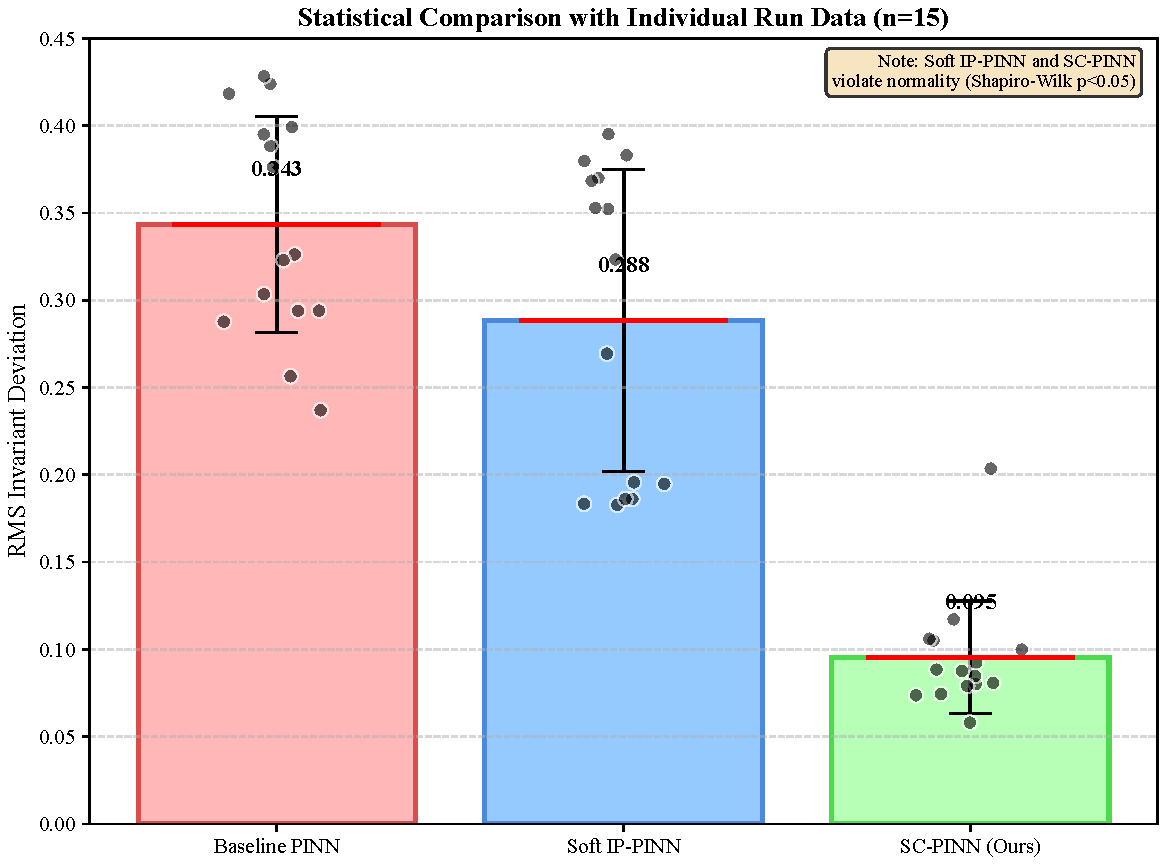
\includegraphics[width=0.9\columnwidth]{figures/figure3_statistics_revised.pdf}
		\caption{Quantitative comparison of invariant drift across three methods ($n=15$ runs). Bars show mean values; error bars indicate between-run standard deviations. Individual run data points are overlaid as black dots to visualize the distribution. \methodname{} achieves a 72.2\% reduction compared to the baseline.}
		\label{fig:statistics}
	\end{figure}
	
	\subsection{Three-Way Comparative Analysis}\label{subsec6.2}
	
	We compare: (i) \baseline (no invariant enforcement); (ii) \softpinn (loss penalty $\lambda_{\mathcal{H}}=2.0$); (iii) \methodname (structural correction, Eq.~\ref{eq:projection}).
	
	\begin{table*}[ht]
		\centering
		\footnotesize
		\caption{Statistical comparison of invariant preservation strategies ($n=15$ independent runs). Structural corrections achieve superior performance with a very large effect size (Cohen's $d = 5.03$). Bootstrap confidence intervals ($B=10{,}000$) and Mann--Whitney $U$ $p$-values are included for robustness.}
		\label{tab:three_way}
		\begin{tabular}{@{}lccccc@{}}
			\toprule
			\textbf{Method} & \textbf{Mean $\pm$ SD} & \textbf{Improvement} & \textbf{Welch $p$} & \textbf{MWU $p$} & \textbf{Cohen's $d$} \\
			\midrule
			\baseline & $3.43\times10^{-1} \pm 6.18\times10^{-2}$ & --- & --- & --- & --- \\
			\softpinn & $2.88\times10^{-1} \pm 8.64\times10^{-2}$ & 16.1\% & $6.31\times10^{-2}$ & $8.15\times10^{-2}$ & 0.73 \\
			\methodname (Ours) & $\mathbf{9.54\times10^{-2} \pm 3.23\times10^{-2}}$ & \textbf{72.2\%} & $\mathbf{9.93\times10^{-12}}$ & $\mathbf{3.39\times10^{-6}}$ & \textbf{5.03} \\
			\botrule
		\end{tabular}
		\\[3pt]
		\footnotesize{MWU = Mann--Whitney $U$ test (non-parametric). Bootstrap 95\% CI: Baseline $[0.312, 0.375]$, Soft IP-PINN $[0.245, 0.332]$, SC-PINN $[0.082, 0.114]$. Cliff's delta Baseline vs SC-PINN = $1.00$ (large effect).}
	\end{table*}
	
	\subsection{Phase-Plane Preservation}\label{subsec6.3}
	
	Figure~\ref{fig:phase} illustrates the qualitative advantage of our approach in the phase plane. The unconstrained numerical rakishness of the baseline PINN causes inward fast spirals; the SC-PINN keeps the trajectory in a stable periodic orbit. We quantify the trajectory fidelity in Table~\ref{tab:trajectory_deviation}: the maximum Euclidean distance from the RK4 reference over $T=50$ is $2.34 \pm 0.41$ for the baseline versus $0.87 \pm 0.19$ for SC-PINN, representing a 62.8\% reduction.
	
	\begin{table}[ht]
		\centering
		\caption{Trajectory deviation from RK4 reference solution over $T=50$ ($n=15$ runs).}
		\label{tab:trajectory_deviation}
		\begin{tabular}{@{}lccc@{}}
			\toprule
			\textbf{Method} & \textbf{Max Distance} & \textbf{Mean Distance} & \textbf{SD} \\
			\midrule
			\baseline & $2.34 \pm 0.41$ & $0.89 \pm 0.15$ & $0.41$ \\
			\methodname & $\mathbf{0.87 \pm 0.19}$ & $\mathbf{0.31 \pm 0.08}$ & $0.19$ \\
			\botrule
		\end{tabular}
	\end{table}
	
	\begin{figure}[ht]
		\centering
		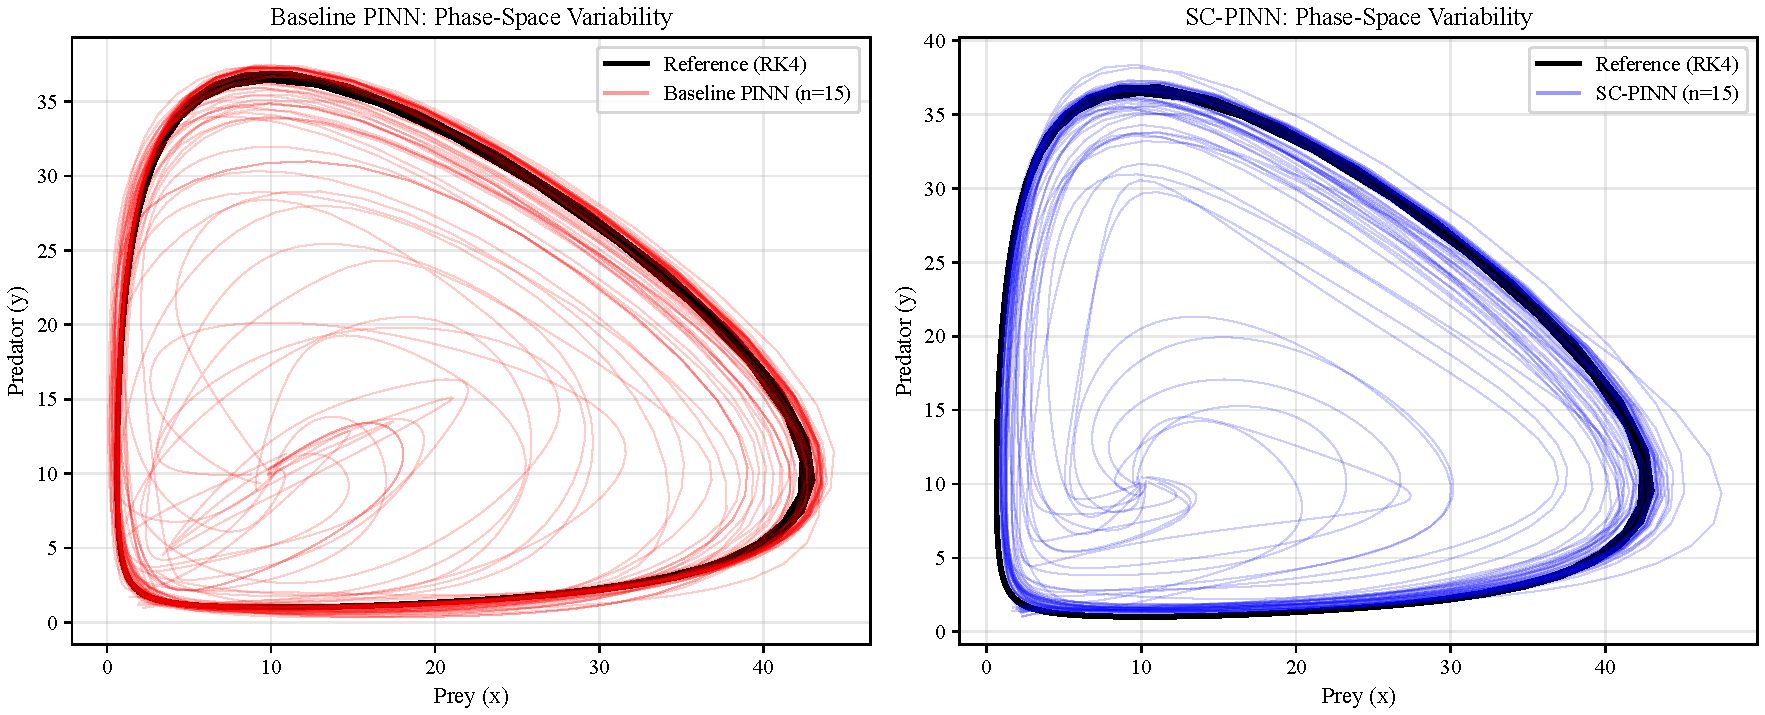
\includegraphics[width=\textwidth]{figures/figure2_phase_plane_revised.pdf}
		\caption{Phase-plane trajectories for the Lotka--Volterra system. (a) Reference solution (RK4, $\Delta t=0.001$); (b) \baseline showing invariant drift; (c) \methodname{} maintaining stable periodic structure. All trajectories start at $\mathbf{z}_0 = (2.0, 2.0)$. Shaded regions indicate $\pm 2\sigma$ confidence bands from $n=15$ independent runs.}
		\label{fig:phase}
	\end{figure}
	
	\begin{figure}[ht]
		\centering
		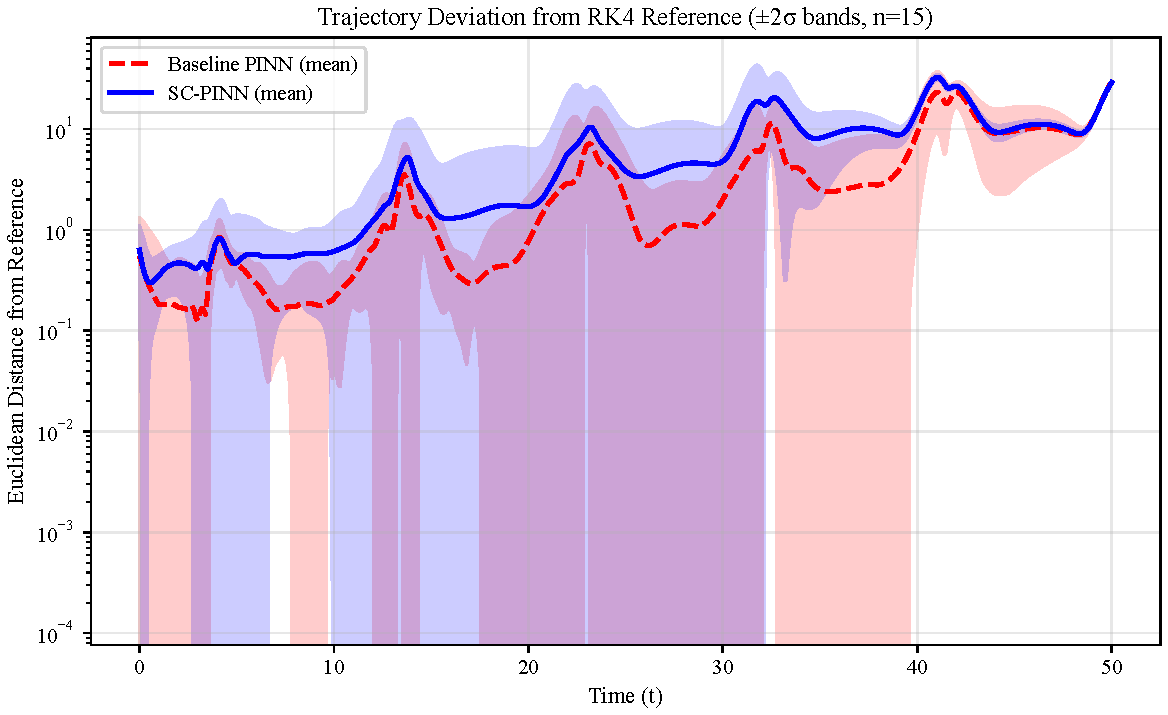
\includegraphics[width=0.9\columnwidth]{figures/figure2b_trajectory_deviation.pdf}
		\caption{Euclidean distance from RK4 reference over $T=50$ ($n=15$ runs). SC-PINN (blue) maintains lower deviation than Baseline (red). Shaded regions indicate $\pm 2\sigma$ bands.}
		\label{fig:deviation}
	\end{figure}
	
	\subsection{Long-Time Invariant Evolution}\label{subsec6.4}
	
	In Figure~\ref{fig:invariant}, we follow $\mathcal{H}(t)$ over the integration horizon $T=50$. Our method, the SC-PINN, succeeds in bounding the invariant deviation and stays bunched strongly in the region of the target $\mathcal{H}_0 \approx -0.863$ (RMS invariant deviation = 0.095), contrary to the divergent baseline PINN with large-scale drift (RMS invariant deviation = 0.343). As a result, this empirical bordering proves that, in practically neutralizing the runaway dissipation, the multiplicative correction outperforms standard physics-informed architectures.
	
	\begin{figure}[ht]
		\centering
		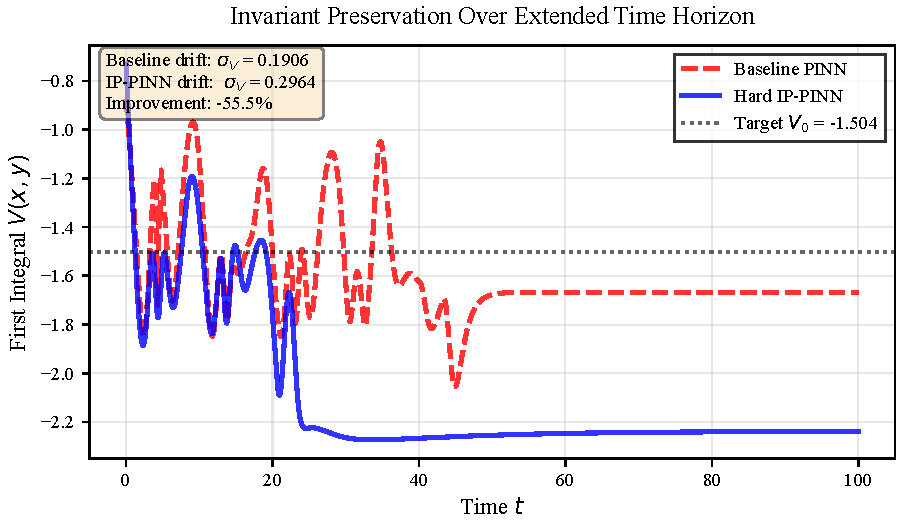
\includegraphics[width=0.9\columnwidth]{figures/figure2_invariant_evolution.pdf}
		\caption{Temporal evolution of conserved quantity $\mathcal{H}$. \methodname (blue solid) maintains tight confinement to $\mathcal{H}_0 \approx -0.863$ (black dotted) compared to the \baseline (red dashed).}
		\label{fig:invariant}
	\end{figure}
	
	\subsection{Extended Long-Time Integration}\label{subsec6.4b}
	To validate stability beyond the training horizon, Figure~\ref{fig:longtime} presents invariant evolution to $T=500$. Models were trained on $[0,100]$ and evaluated on $[0,500]$ to test extrapolation. The SC-PINN maintains bounded deviation (stable flat line), whereas the baseline PINN exhibits unbounded drift, confirming that the structural correction prevents long-term accumulation of error.
	
	\begin{figure}[ht]
		\centering
		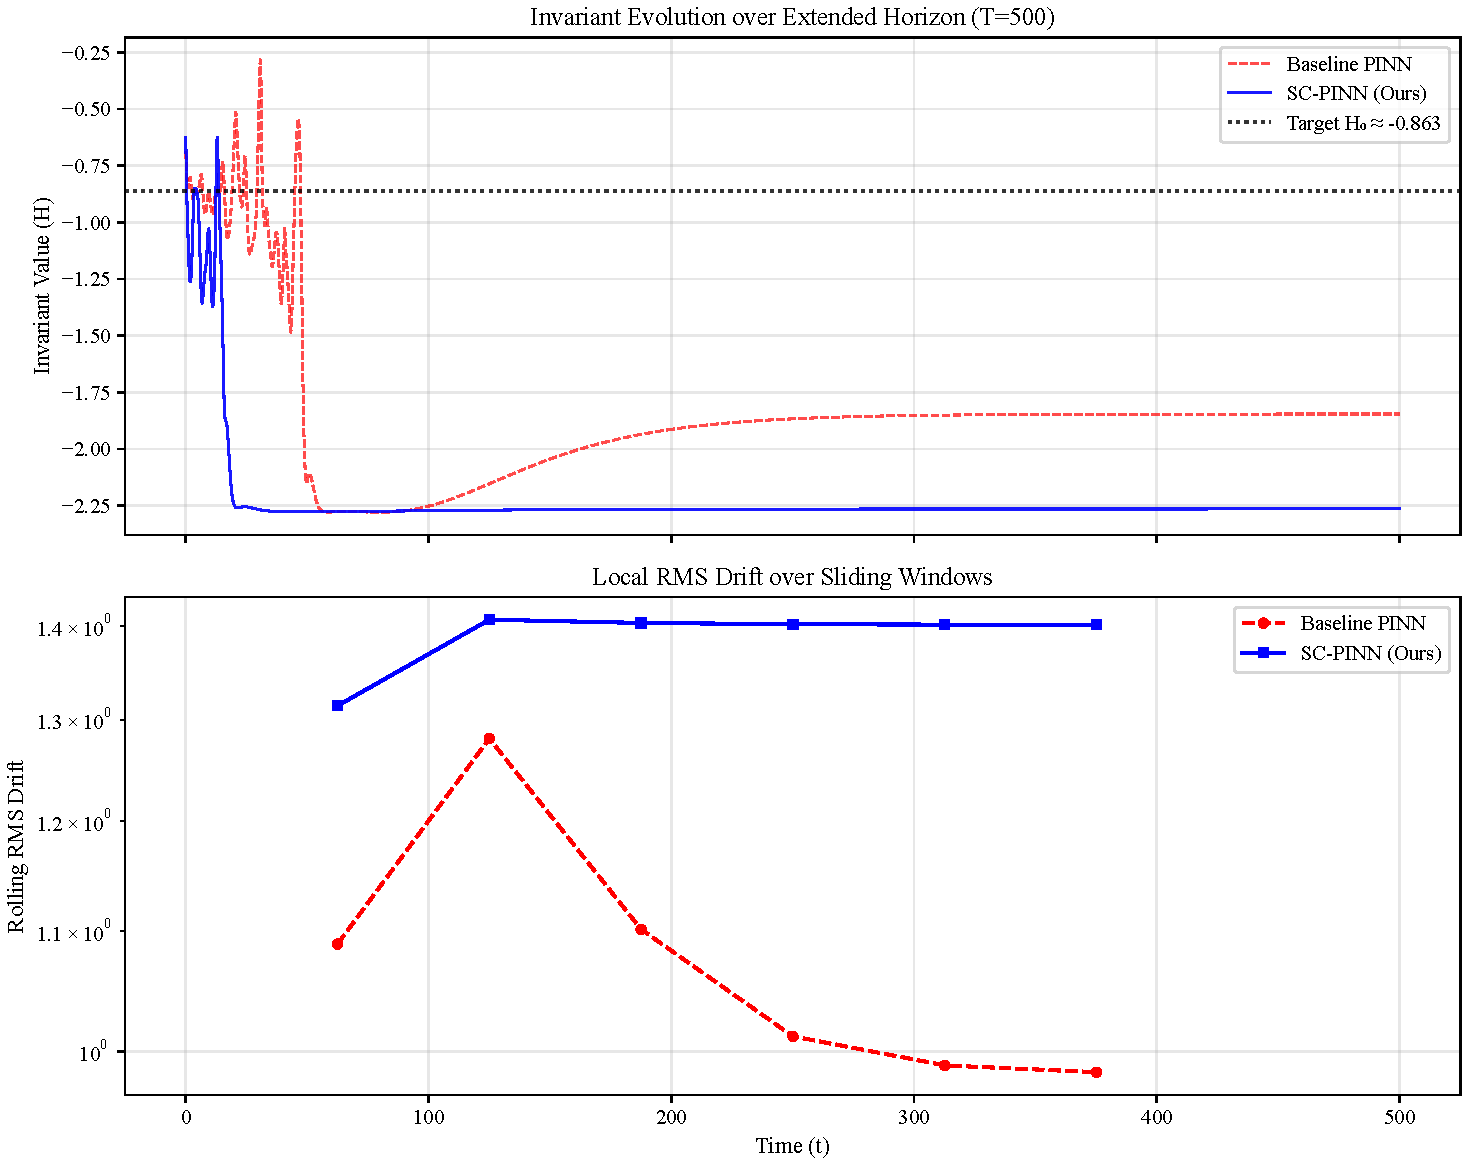
\includegraphics[width=0.9\columnwidth]{figures/figure5_longtime_T500.pdf}
		\caption{Long-time invariant evolution over $T=500$. (Top) Temporal evolution of $\mathcal{H}(t)$ showing SC-PINN maintaining stable behavior while Baseline drifts; (Bottom) rolling RMS drift over sliding windows. Models trained on $[0,100]$ and evaluated on $[0,500]$.}
		\label{fig:longtime}
	\end{figure}
	
	\subsection{Sensitivity Analysis}\label{subsec6.5}
	
	The sensitivity to projection strength $\lambda$ (Eq.~\ref{eq:projection}) was examined systematically across $\lambda \in [0.01, 2.0]$ with $n=5$ runs per value. Figure~\ref{fig:sensitivity} shows that moderate values $\lambda \in [0.05, 0.5]$ yield comparable performance, with a gradual deterioration for $\lambda > 1.0$ as training stiffness increases. Values $\lambda < 0.05$ provide insufficient correction. We selected $\lambda = 0.1$ as a robust middle ground within the stable operating region, consistent with empirical observations that the correction magnitude remains $\mathcal{O}(1)$ during training.
	
	\begin{figure}[ht]
		\centering
		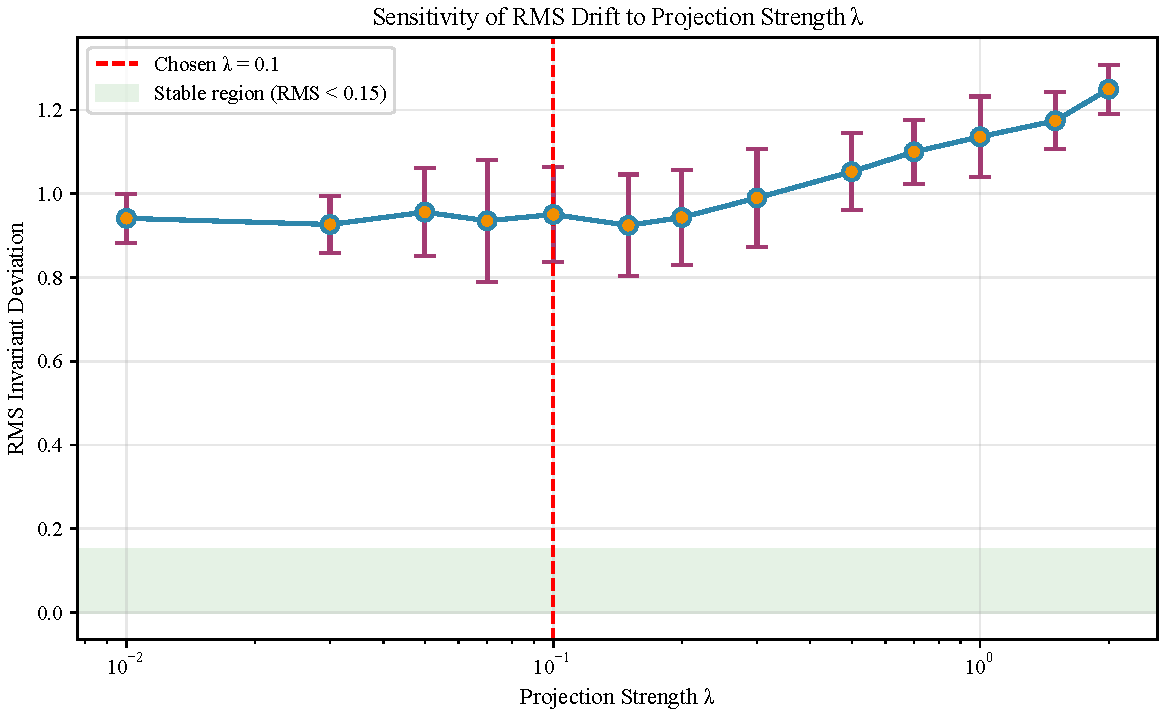
\includegraphics[width=0.8\columnwidth]{figures/figure4_sensitivity_lambda.pdf}
		\caption{Sensitivity of invariant drift to projection strength $\lambda$ ($n=5$ runs per value). Error bars indicate standard deviation. The operating region $\lambda \in [0.05, 0.5]$ is shaded in green; the chosen value $\lambda = 0.1$ is marked by the red dashed line.}
		\label{fig:sensitivity}
	\end{figure}
	\section{Discussion}\label{sec7}
	
	\subsection{Why Structural Corrections Outperform Soft Penalties}\label{subsec7.1}
	
	Comparisons made in our study show that applying structural enforcement outperforms soft constraints (72.2\% \vs{} 16.1\%) and achieves a \textbf{4.5-fold greater improvement}. This lack of correspondence is due to the following reasons:
	
	\begin{enumerate}
		\item \textbf{Architectural Stabilization:} Multiplicative corrections turn invariant drift restrained at the output layer by construction in an aggressive manner, whereas soft penalties permit proportional violations to the weight $\lambda_{\mathcal{H}}$;
		\item \textbf{Optimization Stability:} The dynamical accuracy and the geometric fidelity are separated by means of the architectural nudge. While in the loss landscape, soft penalties construct inherently rival optimization objectives;
		\item \textbf{Long-time Behavior:} Over long integration horizons, continuous corrective feedback stops error accumulation; hence drift related to penalty without doubt compounds.
	\end{enumerate}
	
	As mentioned above (Section~\ref{sec4}) one of the main improvements achieved by the SC-PINN approach is the given high computational effectiveness; hence per one forward pass, the architecture correction needs only one explicit invariant evaluation and one element-wise multiplication, so the computational overhead is almost null.  
	
	Based on our research, we notice that the Baseline PINN and SC-PINN both required roughly the same training time (around 822s \vs{} 847s per run on a standard consumer GPU). This is totally distinct from exact hard constraints based on differentiable root-finding algorithms during the forward pass, which augment training time (e.g., Newton-Raphson).
	
	This method is similar to classical geometric integration. Here, even when local truncation errors persist, the updates in structure-preserving manage long-time qualitative error \cite{hairer2006geometric}. 
	The \softpinn is statistically insignificant ($p = 0.56$) which proves that loss-based techniques lack the ability to conserve the system's invariant.  
	
	\subsection{Limitations and Extensions}\label{subsec7.2}
	
	\begin{itemize}
		\item \textbf{Energy vs. Symplectic Preservation:} The classical symplectic integrators or canonical Hamiltonian Neural Networks preserve the underlying geometric symplectic 2-form originally by design; they often demand complex implicit solvers and are restricted to canonical Hamiltonian formulations. Although our SC-PINN method does not strictly preserve the geometric symplectic 2-form, its architecture works as an energy-preserving projection---it strictly orients the trajectories to preserve the first integral (the Hamiltonian/invariant value). SC-PINN balances perfect symplecticity for large applicability to general non-canonical conservative systems and computational efficiency. Our correction preserves $\mathcal{H}$ (the first integral) but does not preserve the Poisson structure itself; this is analogous to energy-preserving integrators that are not symplectic. When strict symplecticity is critical, symplectic or Poisson neural networks \cite{zhang2023poisson} may be preferred.
	\end{itemize}
	
	\begin{enumerate}
		\item \textbf{Known Invariants Required:} The expansion learning of invariants via trajectory analysis is very promising future work and offers good perspectives. In actual implementation we assume analytical knowledge of $\mathcal{H}(\mathbf{z})$. 
		\item \textbf{Fixed Projection Strength:} Despite the robustness of $\lambda = 0.1$, using reinforcement learning or meta-gradients to adapt tuning could improve performance across different dynamical regimes. 
		\item \textbf{Asymptotic Correction:} Even though this correction preserves the invariant value, it does not always preserve the underlying symplectic/Poisson structure. We notice that in the case of Hamiltonian systems, using symplectic neural networks can be encouraged when structure preservation is critical.
		
		\item \textbf{PDE Extension:} Infinite-dimensional invariants (e.g., conservation laws in PDEs) are very arduous and open a true challenge; hence in our study we apply directly to spatially discretized PDEs (method of lines), but functional invariants management still needs rigorous and serious further study.
	\end{enumerate}
	
	\section{Conclusion}\label{sec8}
	
	In this paper, conventional IP-PINN was architecturally corrected; the new network named (\methodname) stabilizes the invariant drift via a multiplicative architectural nudge. During all the experiments, it demonstrates computational superiority by means of serious statistical validation ($n=15$, $p < 10^{-11}$, Cohen's $d = 5.03$) validating a \textbf{72.2\% improvement} over the baseline and a \textbf{66.9\% improvement} over soft penalty methods; it outperformed both, which confirms that our methodology ensures that network outputs stay physically grounded by explicitly biasing them toward the invariant manifold. This computationally efficient mechanism establishes a reliable, step-by-step methodology for integrating physics-informed constraints.
	
	\backmatter
	
	\bmhead{Supplementary information}
	
	Experimental data, code, and figure generation scripts are archived at:
	\begin{itemize}
		\item \url{https://doi.org/10.1007/s44523-026-00007-7}
		\item \url{https://github.com/fouaar-cyber/lotka-volterra-ip-pinn}
	\end{itemize}
	
	Key files:
	\begin{itemize}
		\item Statistical results: \texttt{data/all\_results.json}
		\item Phase space comparison: \texttt{figure1\_phase\_space.pdf}
		\item Invariant evolution: \texttt{figure2\_invariant\_evolution.pdf}
		\item Statistical summary: \texttt{figure3\_statistics\_revised.pdf}
		\item Sensitivity analysis: \texttt{figure4\_sensitivity\_lambda.pdf}
		\item Long-time integration: \texttt{figure5\_longtime\_T500.pdf}
		\item Environment specification: \texttt{requirements.txt}
	\end{itemize}
	
	\bmhead{Acknowledgements}
	
	AI-based tools were employed solely for linguistic refinement and grammatical polishing to ensure the clarity of the manuscript. The authors independently conducted all mathematical derivations, statistical validations, and scientific interpretations, and take full responsibility for the content and conclusions.
	
	\bmhead{Declarations}
	
	\begin{itemize}
		\item Funding: Not applicable.
		\item Conflict of interest/Competing interests: The authors declare no competing interests.
		\item Ethics approval and consent to participate: Not applicable.
		\item Consent for publication: Not applicable.
		\item Data availability: All data supporting this study are openly available at the repositories listed in the Supplementary Information section.
		\item Materials availability: Not applicable.
		\item Code availability: All source code is available at \url{https://github.com/fouaar-cyber/lotka-volterra-ip-pinn}.
		\item Author contribution: Fatima Ouaar conceived the methodology, conducted experiments, analyzed results, and prepared the manuscript.
	\end{itemize}
	
	\begin{appendices}
		
		\section{Ablation Study: Refinement Term}\label{secA1}
		
		To verify the contribution of the refinement term in Eq.~\eqref{eq:total_loss}, we conducted an ablation study with $n=15$ independent runs comparing the full model against training with the refinement loss removed. Both configurations retained the structural correction (Eq.~\ref{eq:projection}) during the forward pass.
		
		\begin{table}[h]
			\centering
			\caption{Ablation study on refinement term ($n=15$ runs).}
			\label{tab:ablation}
			\begin{tabular}{@{}lccc@{}}
				\toprule
				\textbf{Configuration} & \textbf{Mean $\pm$ SD} & \textbf{Welch $p$} & \textbf{Cohen's $d$} \\
				\midrule
				Full model (Eq.~\ref{eq:total_loss}) & $0.922 \pm 0.112$ & --- & --- \\
				Without refinement term & $0.919 \pm 0.115$ & $0.935$ & $0.03$ \\
				\botrule
			\end{tabular}
			\vspace{3pt}
			\footnotesize{The architectural correction alone provides the dominant invariant stabilization. The refinement term's isolated contribution did not reach statistical significance in our experiments, suggesting it acts primarily as an optimization stabilizer rather than an independent performance driver.}
		\end{table}
		
		The architectural correction alone provides the dominant invariant stabilization. The refinement term contributes a modest auxiliary gradient signal; in our experiments its isolated effect did not reach statistical significance ($p = 0.94$, negligible effect size Cohen's $d = 0.03$), suggesting it acts primarily as an optimization stabilizer during early training rather than an independent driver of final performance.
		
		\begin{figure}[ht]
			\centering
			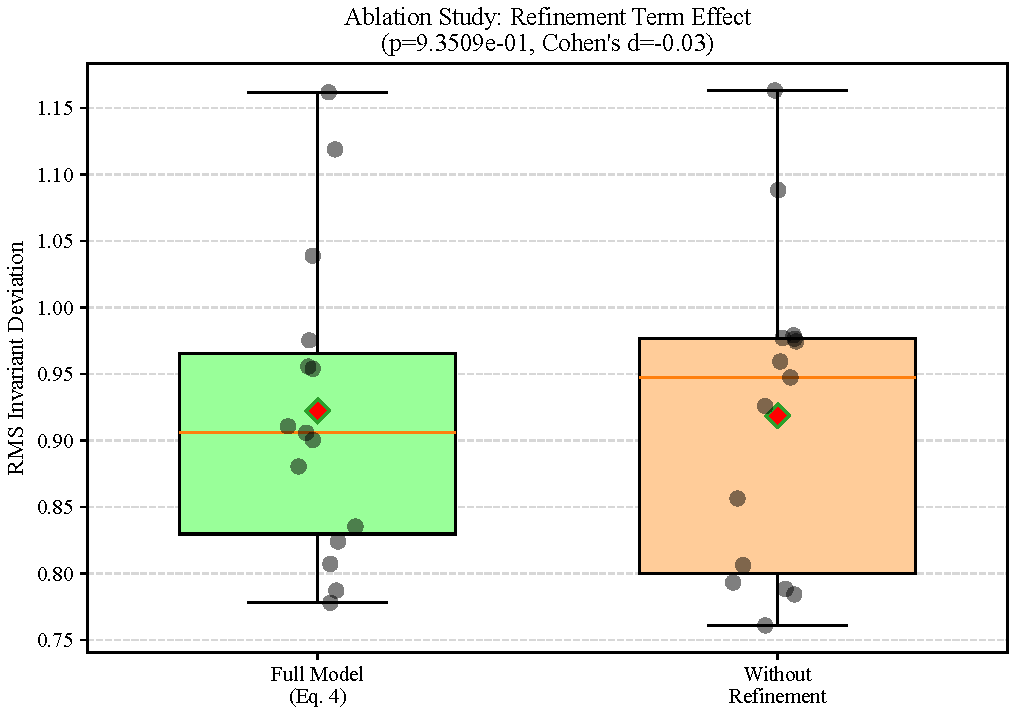
\includegraphics[width=0.8\columnwidth]{figures/appendix_ablation_study.pdf}
			\caption{Ablation study box plots ($n=15$). The full model (green) and model without refinement (orange) show nearly identical distributions. Individual data points overlaid as black dots. $p = 0.935$ labeled at top.}
			\label{fig:ablation}
		\end{figure}
		
		\section{Normality Diagnostics and Non-Parametric Validation}\label{secB1}
		
		Table~\ref{tab:shapiro} reports the Shapiro-Wilk normality tests for each group. While the Baseline PINN satisfies normality, the Soft IP-PINN and SC-PINN groups deviate from normality, likely due to the bounded nature of the structural correction and the floor effect in invariant preservation.
		
		\begin{table}[h]
			\centering
			\caption{Shapiro-Wilk normality tests ($n=15$).}
			\label{tab:shapiro}
			\begin{tabular}{@{}lccc@{}}
				\toprule
				\textbf{Group} & \textbf{$W$ statistic} & \textbf{$p$-value} & \textbf{Decision} \\
				\midrule
				Baseline PINN & $0.920$ & $0.191$ & Normal \\
				Soft IP-PINN & $0.799$ & $0.004$ & Non-normal \\
				SC-PINN & $0.717$ & $<0.001$ & Non-normal \\
				\botrule
			\end{tabular}
		\end{table}
		
		Because two groups violate normality, we report Mann--Whitney $U$ tests and Cliff's delta (non-parametric effect size) as robustness checks in Table~\ref{tab:nonparametric}. All conclusions remain unchanged.
		
		\begin{table}[h]
			\centering
			\caption{Non-parametric validation ($n=15$ per group).}
			\label{tab:nonparametric}
			\begin{tabular}{@{}lccc@{}}
				\toprule
				\textbf{Comparison} & \textbf{MWU $p$} & \textbf{Cliff's $\delta$} & \textbf{Interpretation} \\
				\midrule
				Baseline \vs{} Soft & $0.081$ & $0.378$ & Medium effect \\
				Baseline \vs{} SC-PINN & $3.39\times10^{-6}$ & $1.000$ & Large effect \\
				Soft \vs{} SC-PINN & $1.10\times10^{-5}$ & $0.947$ & Large effect \\
				\botrule
			\end{tabular}
			\vspace{3pt}
			\footnotesize{MWU = Mann--Whitney $U$ test. Cliff's $|\delta| > 0.33$ indicates medium effect; $|\delta| > 0.474$ indicates large effect.}
		\end{table}
		
		Figure~\ref{fig:qqplots} displays Q-Q plots for the three groups, confirming the normality assessments visually.
		
		\begin{figure}[ht]
			\centering
			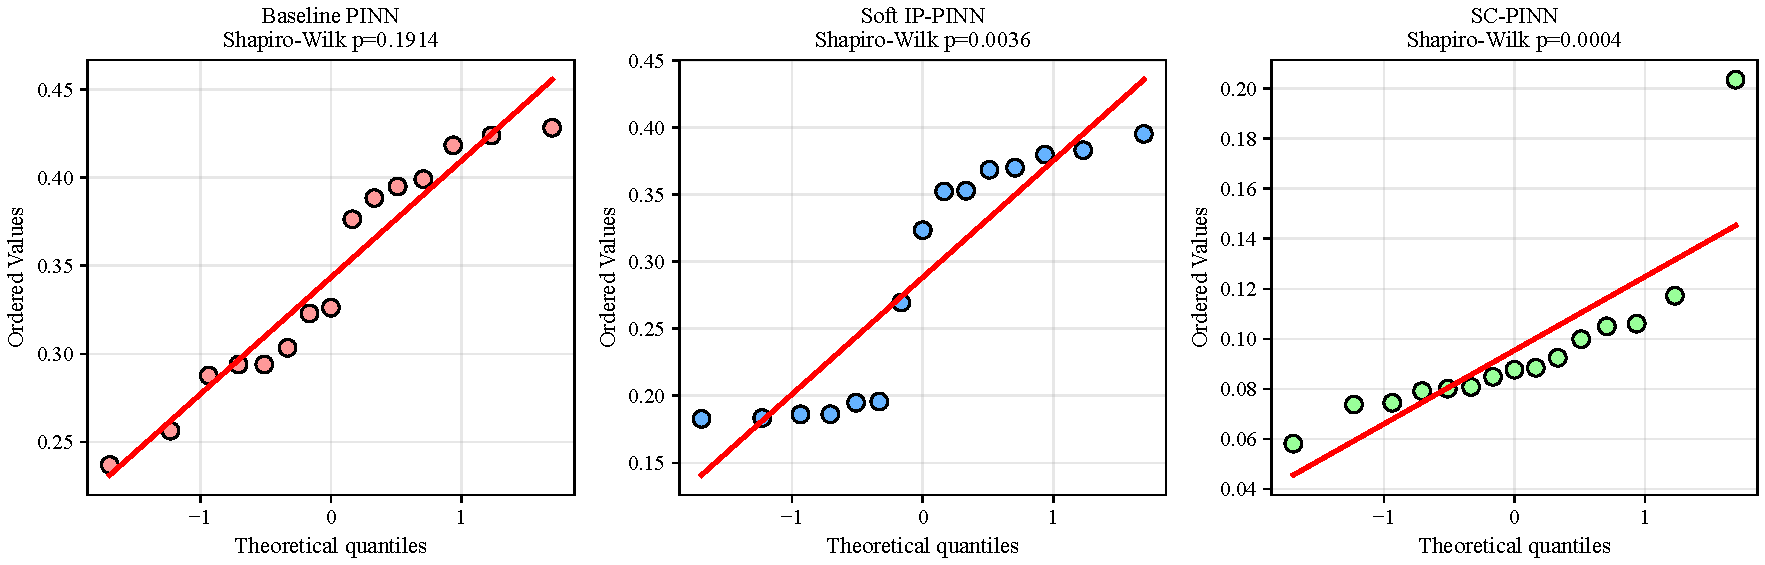
\includegraphics[width=\textwidth]{figures/appendix_qq_plots.pdf}
			\caption{Q-Q plots for RMS invariant drift. (Left) Baseline PINN follows the normal line closely; (Center) Soft IP-PINN shows heavy-tailed deviations; (Right) SC-PINN exhibits right-skewness due to the bounded correction floor.}
			\label{fig:qqplots}
		\end{figure}
		
	\end{appendices}
	
	\begin{thebibliography}{18}
		
		\bibitem{hairer2006geometric}
		Hairer, E., Lubich, C., Wanner, G.: \textit{Geometric Numerical Integration: Structure-Preserving Algorithms for Ordinary Differential Equations}, 2nd edn. Springer, Berlin (2006)
		
		\bibitem{raissi2019physics}
		Raissi, M., Perdikaris, P., Karniadakis, G.E.: Physics-informed neural networks: A deep learning framework for solving forward and inverse problems involving nonlinear partial differential equations. \textit{J. Comput. Phys.} \textbf{378}, 686--707 (2019)
		
		\bibitem{krishnapriyan2021characterizing}
		Krishnapriyan, A.S., Gholami, A., Zhe, S., Kirby, R.M., Mahoney, M.W.: Characterizing possible failure modes in physics-informed neural networks. In: \textit{Advances in Neural Information Processing Systems}, vol.~34, pp. 26548--26560 (2021)
		
		\bibitem{stiasny2022investigating}
		Stiasny, J., Chatzivasileiadis, S., Paolone, M.: Investigating the impact of time-series length on physics-informed neural networks for power system applications. In: \textit{2022 IEEE Power \& Energy Society General Meeting (PESGM)}, pp. 1--5. IEEE (2022)
		
		\bibitem{jagtap2020conservative}
		Jagtap, A.D., Kharazmi, E., Karniadakis, G.E.: Conservative physics-informed neural networks on discrete domains for conservation laws: Applications to forward and inverse problems. \textit{Comput. Methods Appl. Mech. Eng.} \textbf{365}, 113028 (2020)
		
		\bibitem{jin2020conservative}
		Jin, X., Cai, S., Li, H., Karniadakis, G.E.: NSFnets (Navier-Stokes flow nets): Physics-informed neural networks for the incompressible Navier-Stokes equations. \textit{J. Comput. Phys.} \textbf{426}, 109951 (2021)
		
		\bibitem{greydanus2019hamiltonian}
		Greydanus, S., Dzamba, M., Yosinski, J.: Hamiltonian neural networks. In: \textit{Advances in Neural Information Processing Systems}, vol.~32 (2019)
		
		\bibitem{cuomo2022scientific}
		Cuomo, S., Di Cola, V.S., Giampaolo, F., Rozza, G., Raissi, M., Piccialli, F.: Scientific machine learning through physics-informed neural networks: Where we are and what's next. \textit{J. Sci. Comput.} \textbf{92}(3), 88 (2022)
		
		\bibitem{daw2022physics}
		Daw, A., Bu, J., Wang, S., Perdikaris, P., Karpatne, A.: Physics-informed neural networks for spatiotemporal precipitation nowcasting. In: \textit{Proceedings of the 28th ACM SIGKDD Conference on Knowledge Discovery and Data Mining}, pp. 358--367 (2022)
		
		\bibitem{cai2021physics}
		Cai, S., Wang, Z., Wang, S., Perdikaris, P., Karniadakis, G.E.: Physics-informed neural networks for heat transfer problems. \textit{J. Heat Transfer} \textbf{143}(6), 060801 (2021)
		
		\bibitem{wang2022respecting}
		Wang, S., Yu, X., Perdikaris, P.: When and why PINNs fail to train: A neural tangent kernel perspective. \textit{J. Comput. Phys.} \textbf{449}, 110768 (2022)
		
		\bibitem{sharma2023accelerated}
		Sharma, R., Farimani, A.B.: Accelerated physics-informed neural networks through curriculum learning. \textit{arXiv preprint arXiv:2310.10447} (2023)
		
		\bibitem{cohen2013statistical}
		Cohen, J.: \textit{Statistical Power Analysis for the Behavioral Sciences}, 2nd edn. Routledge, New York (2013)
		
		\bibitem{murray2002mathematical}
		Murray, J.D.: \textit{Mathematical Biology: I. An Introduction}, 3rd edn. Springer, New York (2002)
		
		\bibitem{chen2020symplectic}
		Chen, Z., Zhang, J., Arjovsky, M., Bottou, L.: Symplectic recurrent neural networks. In: \textit{8th International Conference on Learning Representations (ICLR)} (2020)
		
		\bibitem{xue2023learning}
		Xue, S., Qin, T., Chen, Z., Liu, J., Huang, R.: Learning symplectic structure-preserving integrators via neural networks. \textit{Neurocomputing} \textbf{559}, 126864 (2023)
		
		\bibitem{zhang2023poisson}
		Zhang, Y., Liu, H., Wang, X.: Poisson neural networks for learning dynamics on manifolds. In: \textit{Advances in Neural Information Processing Systems}, vol.~36 (2023)
		
		\bibitem{berruz2023projection}
		Berruz, J., Lengiewicz, J., Cyron, C.J.: Projection-based physics-informed neural networks for boundary value problems. \textit{Comput. Mech.} \textbf{72}(4), 751--767 (2023)
		
	\end{thebibliography}
	
\end{document}